%============================================================================
\begin{table}
\centering
\caption{Galaxy Parameters of J1331.}
\begin{tabular}{lllr}
\hline
redshift \citep{SWELLSIII}                 & $z_d$ & 0.113 \\
angular diameter distance & $D_d$ [Mpc] & 414 \\
scaling                   & 1 kpc / 1 $''$ & 2.006 \\
position angle from North          & $\phi$ [degrees] & $42.90^\circ$\\
average axis ratio & $q'$ & 0.598\\
average ellipticity & $\epsilon = 1 - q'$ & 0.402 \\
apparent I-band magnitude & $m_\text{I}$ [mag] & 15.77 \\
total I-band luminosity & $L_\text{tot,I}$ [$10^{10} L_\odot$] & 5.6 \\
effective half-light radius & $R_\text{eff}$ [$''$] & 2.6 \\
& $R_\text{eff}$ [pc]& 5.2 & \\
\hline
\end{tabular}
\label{tab:galaxyparameters}
\end{table}
%============================================================================

\subsection{Surface photometry for J1331 with MGEs} \label{sec:MGE_results}

In this section we construct a model for the J1331's intrinsic light distribution in terms of MGEs (see Section \ref{sec:MGE_theo}). We use the HST image in the F814W (I-band) filter (Figure \ref{fig:F814W}) because J1331's central stellar component appears at longer wavelengths (i) smoother and more extended than in the F450W filter (Figure \ref{fig:F450W}), as it is less sensitive to young clumpy star-forming regions, (ii) much brighter than the bluish lensing images, and (iii) the imaging is less prone to extinction.

\paragraph{PSF for the HST/F814W filter.} The one-dimensional MGE in Equation \eqref{eq:PSFgeneral} is fitted to the radial profile of a synthetic image of the HST/F814W filter PSF, ignoring diffraction spikes and using the code by \citet{Cap02}. The MGE parameters of the normalized PSF model are given in Table \ref{tab:PSFMGEF814W}.

%============================================================================
\begin{table}
\centering
\caption{F814W PSF MGE: Parameters of the circular four-Gaussian MGE in Equation \eqref{eq:PSFgeneral} fitted to the radial profile of the synthetic HST/F814W PSF image.}
\begin{tabular}{ccc}
\hline
$j$ & $G_j$ & $\delta_j$ [$''$] \\\hline
1 & 0.184 & 0.038\\
2 & 0.485 & 0.085\\
3 & 0.222 & 0.169\\
4 & 0.109 & 0.487\\\hline
\end{tabular}
\label{tab:PSFMGEF814W}
\end{table}
%============================================================================

\paragraph{MGE for the inner regions.} We fit a MGE to J1331's smooth central region within $\sim 5''$ from the HST/WFPC2/WF3/F814W image (Figure \ref{fig:F814W}). Bright objects close to the bulge (blobs possibly belonging to the background galaxy and parts of the foreground spiral arm) were masked during the fit. J1331's galaxy center, position angle (with respect to North through East) and average apparent ellipticity (see Table \ref{tab:galaxyparameters}) are found from the images weighted first and second moment. The MGE fit splits the image in annuli with the given ellipticity and position angle and sectors of $5^\circ$ width and fits an 5-Gaussian MGE of the form in Equation \eqref{eq:MGEgeneral} convolved with the PSF MGE in Table \ref{tab:PSFMGEF814W} to it. The best fit MGE (PSF convolved) is compared to the data in Figure \ref{fig:MGEinnerRegions} and the corresponding parameters of the intrinsic surface brightness distribution are given in Table \ref{tab:MGEF814W}. The fit is a very good representation of the light distribution in the inner $5''$, but underestimates the light distribution outward.

\paragraph{MGE for the outer regions.} To get a handle on the light distribution also in the outer parts of J1331, where spiral arms dominate, we first fit a IRAF \citep{1993ASPC...52..173T} \emph{ellipse} model to the F814W image (masking the brightest blobs in the spiral arms and outer regions). Only then we fit a 7-Gaussian MGE to the smooth ellipse model. The MGE does not perfectly reproduce the flatness of the ellipse model at every radius (see Figure \ref{fig:MGEouterRegions}), but considering the spiral arm dominated outer regions of J1331, it is good enough for an approximate handling of the overall light distribution.

\paragraph{Transformation into physical units.} To transform the MGE in units of counts into physical units, we apply a simplified version of the procedure described in \citet{Holtzman}.

%============================================================================
\begin{figure*}
\centering
\begin{subfigure}{.5\textwidth}
  \centering
  \includegraphics[width=.8\columnwidth]{fig/1331F814Wsci_MGE_M.ps}
  \caption{MGE for J1331's inner regions.}
 \label{fig:MGEinnerRegions}
\end{subfigure}%
\begin{subfigure}{.5\textwidth}
  \centering
  \includegraphics[width=.8\columnwidth]{fig/1331F814W_MGE_disk_L.ps}
  \caption{MGE for J1331's outer regions.}
 \label{fig:MGEouterRegions}
\end{subfigure}%
\caption{MGEs for J1331's surface brightness distribution. Comparison of contours with constant F814W surface brightness (orange lines) with the corresponding iso-brightness contours of the best fit MGE, convolved with the PSF in Table \ref{tab:MGEF814W}, (gray lines). The black line has a length of $10''$ and it's orientation corresponds to the galaxy's position angle as found in Table \ref{tab:galaxyparameters}. For comparison the Einstein radius as found in Table \ref{tab:bestfitlensmodel}  is indicated as red dashed line. \emph{Panel (a)} Central regions of J1331. The MGE model is a good representation of the galaxy's light distribution along the major axis within $\sim 5''$. Its parameters are given in Table \ref{tab:MGEF814W}. This MGE is used as model for the stellar tracer distribution in the dynamical Jeans modelling in Sections \ref{sec:results_JAM_SB} and \ref{sec:results_JAM_NFW}. \emph{Panel (b)} Outer regions of J1331. The orange lines indicate here contours of a smooth IRAF \emph{ellipse} fit to J1331 in the F814W filter; the gray lines are the corresponding best fit MGE. The green box corresponds to the image section shown in Panel (a). This MGE is not used for dynamical modelling, because the dynamics in the outer regions are strongly affected by non-axisymmetries (e.g., spiral arms). We use it, however, to estimate the galaxy's total luminosity and effective radius, and to get a prediction for the dynamics of the outer regions.}
\end{figure*}
%============================================================================

%============================================================================
\begin{table*}
\centering
\caption{Parameters of the best fit MGE to the F814W surface brightness of J1331 in Figure \ref{fig:MGEinnerRegions}. The fit is best inside an radius of $5''$. The position angle is given in Table \ref{tab:galaxyparameters}. This MGE is used in the dynamical modelling in Sections \ref{sec:results_JAM_SB} and \ref{sec:results_JAM_NFW}. The first column gives for each Gaussian the total F814W luminosity in Equation \eqref{eq:centralItotalL} in units of counts. The second column is the corresponding I-band peak surface brightness in Equation \eqref{eq:MGEgeneral} in units of a luminosity surface density. The third and fourth column give the dispersion and the last column the axis ratio of the Gaussian in Equation \eqref{eq:MGEgeneral}.}
\begin{tabular}{cccccc}
\hline
 & total luminosity  & surface density & \multicolumn{2}{c}{Gaussian dispersion} & axis ratio\\
$i$  & $L_i$ [counts] & $I_{0,i}$ [$L_\odot$/pc$^2$] & $\sigma_i$ [$''$] & $\sigma_i$ [kpc] & $q'_i$\\\hline
1  &     9425.96 &      20768.  &  0.051   & 0.103  & 1.00\\
2  &    13173.0 &        3161.2 &  0.178   & 0.358  & 0.76\\
3  &    40235.0 &        1588.2 &  0.503   & 1.008  & 0.58\\
4  &    67755.2 &         502.25&  1.180   & 2.368  & 0.56\\
5  &    203677. &         136.51&  3.891   & 7.805  & 0.57\\\hline
\end{tabular}
\label{tab:MGEF814W}
\end{table*}
%============================================================================

The scaling of the drizzled HST/WFC3 images is  $S \equiv 0.05''/\text{pixel width}$ and the total exposure time $T = 1600$ sec. Each Gaussian in the MGE has a total F814W luminosity $L_i$ (in counts) and a central surface brightness (in counts per pixel) of
\begin{equation*}
C_{0,i}\text{[counts/pixel]} = \frac{L_i[\text{counts}]}{2\pi \sigma[\text{pixel}]^2 q}.
\end{equation*}
This is then transformed into an I-band surface brightness (in $\text{mag}\times(1'')^{-2}$) via
\begin{equation}
\mu_{I,0,i} \simeq -2.5 \log_{10}\left( \frac{C_{0,i}\text{[counts/pixel]}}{T[\text{sec}] \cdot S[''/\text{pixel width}]^2}\right) + Z + C + A_I, \label{eq:muI_}
\end{equation}
where $Z\simeq21.62~\text{mag}$ is a the zero-point from \citet{Holtzman}, updated according to \citet{Dolphin,DolphinNew}, for the photometric system of the HST/WFPC2 camera and the F814W filter, plus a correction for the difference in gain between calibration and observation. $C= 0.1~\text{mag}$ corrects for the finite aperture of the WFPC2; and $A_I =0.015~\text{mag}$ is the extinction in the (Landolt) I-band towards J1331, according to the NASA/IPAC Extragalactic Database (NED)\footnote{The NASA/IPAC Extragalactic Database (NED, \url{https://ned.ipac.caltech.edu/}) is operated by the Jet Propulsion Laboratory, California Institute of Technology, under contract with the National Aeronautics and Space Administration. The data for J1331 (SDSS J133140.33+362811.9) was retrieved in October 2013.}. The color-dependent correction between the F814W filter and the I-band of the UBVRI photometric system is  small \citep{Holtzman} and we neglect it therefore. The last step is to transform the surface brightness $\mu_{I,0,i}$ (in mag) to the I-band surface density $I_{0,i}$ (in $L_\odot$/pc$^2$) of the Gaussian, i.e.,
\begin{eqnarray*}
I_{0,i}[L_\odot \text{pc}^{-2}] = \left( 64800/\pi\right)^2 \left(1+z_d \right)^4 10^{0.4\left(M_{\odot,I}-\mu_{I,0,i} \right)},
\end{eqnarray*}
where the term with $z_d$ accounts for redshift dimming and $M_{\odot,I}=4.08~\text{mag}$ is the Sun's absolute I-band magnitude \citep{1998gaas.book.....B}. The luminosity $L_i$[counts] and the corresponding surface brightness density $I_{0,i} [L_\odot \text{pc}^{-2}]$ of each Gaussian are given in Table \ref{fig:MGEinnerRegions}.

\paragraph{Inclination.} To estimate the inclination of J1331 with respect to the observer, we use the observed axis ratio of the flattest ellipse in the IRAF \emph{ellipse} model for J1331, which is $q'=0.42$. This is similar to the disk axis ratio of $q' = 0.40$ found by \citet{SWELLSI}. If a typical thickness of an oblate disk is around $q_0 \sim 0.2$ \citep{1958MeLu2.136....1H}, the inclination follows from 
\begin{equation*}
\cos^2 i = \frac{q'^2 - q_0^2}{1 - q_0^2}
\end{equation*}
and a correction of $+3^\circ$ \citep{1988ngc..book.....T}. Our estimate for the inclination is therefore $i \approx 70^\circ$. Given this inclination, the 2D MGE models can be deprojected into three dimensions (see Section \ref{sec:MGE_theo}).

\paragraph{Total luminosity and effective radius.} J1331's total I-band luminosity is determined by summing up the luminosity contributions of all the MGE Gaussians for the outer regions (shown as gray lines in Figure \ref{fig:MGEouterRegions}). We find $L_\text{tot,I} \simeq 5.6 \cdot 10^{10} ~L_\odot$. This corresponds to an apparent magnitude of $m_I = 15.77~\text{mag}$. We determine the circularized effective radius $R_\text{eff}$ of J1331 from the definition $L(<R_\text{eff}) \equiv \frac 12 L_\text{tot}$ and the growth curve $L(<R')$ from the MGE model of the outer regions, where $R'$ is the projected radius on the sky. We find the effective radius to be $R_\text{eff} \simeq 2.6'' \hat{=} 5.2 \text{ kpc}$.  All values are summarized in Table \ref{tab:galaxyparameters}.


